\documentclass[10pt]{ctexart}
\usepackage[utf8]{inputenc}
\usepackage[T1]{fontenc}
\usepackage{amsmath}
\usepackage{amsfonts}
\usepackage{amssymb}
\usepackage{mhchem}
\usepackage{stmaryrd}
\usepackage{hyperref}
\usepackage{type1cm}
\usepackage{times}
\usepackage{float}
\usepackage{subfigure}
\usepackage[marginal]{footmisc}
\renewcommand{\thefootnote}{}
\hypersetup{colorlinks=true, linkcolor=blue, filecolor=magenta, urlcolor=cyan,}
\urlstyle{same}
\usepackage{graphicx}
\usepackage[export]{adjustbox}
\graphicspath{ {./images/} }

\title{工业应用中LoRa和ZigBee的性能分析 $4.0$ }


\author{Renan R. Mendes, Rafael M. Silva, Carlos E. Capovilla\\
and Ivan R. S. Casella \\
Federal University of ABC, Santo Andre, SP, Brazil\\
\{renan.mendes, carlos. capovilla, ivan. casella $\}$@ufabc.edu.br,\\
r.montoia@aluno.ufabc.edu.br}
\date{}

\begin{document}
\maketitle


\begin{abstract}
工业4.0概念已经在全球范围内逐步得到巩固,它的成功很大程度上归功于LPWA通信技术的应用。其中,LoRa和Zigbee脱颖而出,除了低功耗和覆盖范围大的特点,它们成本低,并且使用扩频技术来增加系统对干扰的鲁棒性。在此背景下,本文对这两个技术在室内和室外环境中的性能进行了研究,以分析它们在工业4.0中使用的可行性。
\end{abstract}

关键词: Industry 4.0·IoT·LPWA·LoRa·Zigbee

\section{简介}
近年来,世界工业经历了一场真正的革命。工业4.0的概念已被部署用于提供物联网(IoT)技术,用于监控和控制工业过程[1]。其快速增长的一个原因是采用无线LPWA(低功率广域)通信技术。 其中,LoRa(远距离)和Zigbee技术已显示出广阔的前景,因为它们提供的设备价格实惠,易于获取,部署成本低且具有良好的抗干扰能力(扩频技术),此外还有低功耗(例如,大约10年)和远程(例如,几公里)[2-4]。 

目前成功实施工业4.0概念的一个非常重要的问题,是这些技术在不同的无线电传播环境中的性能,例如部署在那些工业厂房中时。因此,最近在科学文献中发表了几篇作品 [1,5-7]。

在此背景下,本文旨在基于在室内和室外环境中进行的实验获得的测量数据,对LoRa和Zigbee技术进行比较研究,以验证它们在工业4.0中的可行性。分析将使用RSSI(接收信号强度指示)、PER(数据包错误率)的测量值和估计的最大范围作为性能参考。

除引言外,本文还分为四个部分。第2节简要介绍了待评估的技术——LoRa和Zigbee。第3节展示了测量测试的方式。第4节展示了无线电传播模型分析。最后第5节对全文进行了总结。

\footnote{\copyright The Author(s), under exclusive license to Springer Nature Switzerland AG 2021\\ 
Y. Iano et al. (Eds.): BTSym 2020, SIST 233, pp. 801-810, $2021 .$\\
\href{https://doi.org/10.1007/978-3-030-75680-2_89}{https://doi.org/10.1007/978-3-030-75680-2\_89}
}

\section{技术概述}
LoRa使用Chirp扩频(CSS),并已指定在某些特定的ISM(工业、科学和医疗)频段上运行。本文中,选择了$915\mathrm{MHz}$频段标准,因为这是LoRa在巴西采用的频段。LoRa有一个非常有趣的特性:它允许对系统的一些重要参数进行调整,例如SF(扩频因子,从7到12)、BW(带宽,从125到$500\mathrm{kHz}$)和CR(编码速率,从$4/5$到$4/8$)[8]。根据这些参数,数据速率可以从$0.3$到$50\mathrm{kbps}$不等。

另一方面,Zigbee采用直接序列扩频(DSSS)。它已被标准化在三个不同的ISM频段上运行,每个频段都有非常不同的特性[9]。本文中,将采用$2.4\mathrm{GHz}$标准,因为它是在巴西最常用的标准。它采用基于OQPSK(偏移四进制相移键控)的准正交调制,可以实现大约250kbps[6]的数据速率。

\section{性能分析}
本文旨在从传输质量(RSSI和PER)和传输范围的角度评估和比较LoRa和Zigbee技术的性能。由于工业厂房的特性,系统的性能将针对室内和室外环境进行分析。

对于LoRa性能分析,使用了两个基于SX$1276$芯片的ESP-LoRa设备,工作在$915\mathrm{MHz}$,距离地面$2.0\mathrm{~m}$,其中一个用作发射器(TX)和另一个作为接收器(RX)。该研究基于表$1$中针对SF、BW和传输功率$\left(P_{TX}\right)[1]$的不同可能组合给出的八种可能的LoRa操作配置。

对于Zigbee性能分析,使用了两个运行在$2.4\mathrm{GHz}$的Xbee-Pro设备(TX和RX)。每个设备都连接到一个嵌入式Arduino Mega系统,用于控制和传输数据包,并且与LoRa测试一样,两者都位于距离地面$2.0\mathrm{~m}$的位置。

$\footnote{\text{https://semtech.com/products/wireless-rf/lora-transceivers/sx } 1276 .}$

\subsection{室内环境}
室内环境测试在圣安德烈的$\mathrm{ABC}$联邦大学(UFABC)A楼的地下室进行。从RSSI和PER参数的测量结果分析LoRa和Zigbee的性能。

在测量期间,TX保持固定,RX从$10\mathrm{~m}$开始移动,每次移动$10\mathrm{~m}$,直到达到$100\mathrm{~m}$。重要的是要注意,系统在站点上会受到不同的干扰,例如来自运行中的WiFi(无线保真)网络的同信道干扰。专门针对LoRa,对表$1$中列出的所有配置进行了测量。

\begin{table}
  \centering
  \renewcommand{\tablename}{表}
  \caption{LoRa 配置}
  \begin{tabular}{l|l|l|l}
    \hline
    配置 & SF & BW $(\mathrm{kHz})$ & $P_{T X}(\mathrm{dBm})$ \\
    \hline
    Config 1 & 7 & 125 & 14 \\
    \hline
    Config 2 & 12 & 125 & 14 \\
    \hline
    Config 3 & 7 & 125 & 20 \\
    \hline
    Config 4 & 12 & 125 & 20 \\
    \hline
    Config 5 & 7 & 500 & 14 \\
    \hline
    Config 6 & 12 & 500 & 14 \\
    \hline
    Config 7 & 7 & 500 & 20 \\
    \hline
    Config 8 & 12 & 500 & 20 \\
    \hline
  \end{tabular}
\end{table}

进行测试的室内环境如图$1$所示。

\begin{figure}[H]
  \centering
  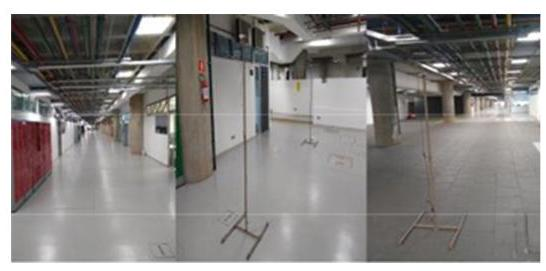
\includegraphics[max width=\textwidth]{2022_02_28_100dc43db44c8290ce2ag-03}
  \renewcommand{\figurename}{图}
  \caption{室内环境}
\end{figure}


图2显示了所分析室内环境的RSSI变化作为$d$(距离)的函数,可以看出,对于LoRa,RSSI的测量值在$-60$和$-96\mathrm{dBm}$之间。对于Zigbee可以看出,在小于$50\mathrm{~m}$时,RSSI高于$-50\mathrm{dBm}$,而在$50\mathrm{~m}$以上,RSSI高于$-65\mathrm{dBm}$。

\begin{figure}[H]
  \centering
  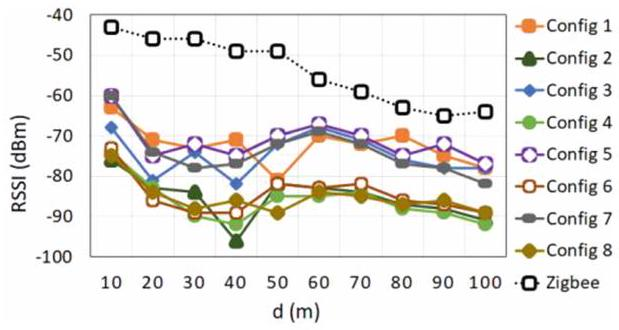
\includegraphics[max width=\textwidth]{2022_02_28_100dc43db44c8290ce2ag-04}
  \renewcommand{\figurename}{图}
  \caption{RSSI作为室内环境中$d$的函数}
\end{figure}

反过来,图3显示了在分析的室内环境中,对于Lora(配置1和配置6)和Zigbee,PER作为$d$(距离)的函数的结果。在测试中,定义了三个不同的测量点$(10,50$,和$100\mathrm{~m})$,并且在每个点上传输了$10.000$的数据包。可以看出,在高达$100\mathrm{~m}$的情况下,LoRa对Config 1的最大PER为$2.2\%$,对Config 6的最大PER为$1.8\%$。对于Zigbee,最大PER在$10\mathrm{~m}$和$50\mathrm{~m}$之间为$0.4\%$。然而,对于$100\mathrm{~m}$,PER有显着增加,约为$22.5\%$。

\begin{figure}[H]
  \centering
  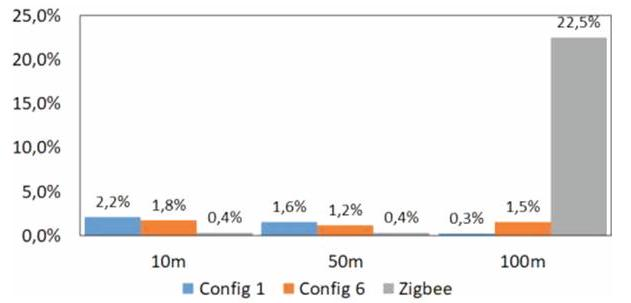
\includegraphics[max width=\textwidth]{2022_02_28_100dc43db44c8290ce2ag-04(1)}
  \renewcommand{\figurename}{图}
  \caption{PER作为室内环境中$d$的函数}
\end{figure}

\subsection{室外环境}

室外测量在圣贝尔纳多-杜坎波工学院(FATEC)进行。图4显示了执行测试的环境。在测量过程中,TX保持固定,RX放置在距离TX$100$、$200$、$250$和$300\mathrm{~m}$的位置,两者的高度均为$2.0\mathrm{~m}$。为简单起见,LoRa测量仅针对Config 1和Config 6进行。图5显示了测量点($a$)和地形的高程剖面($b$)。可以看出TX和RX之间的最大斜率为$22.0\mathrm{~m}$。

\begin{figure}[H]
  \centering
  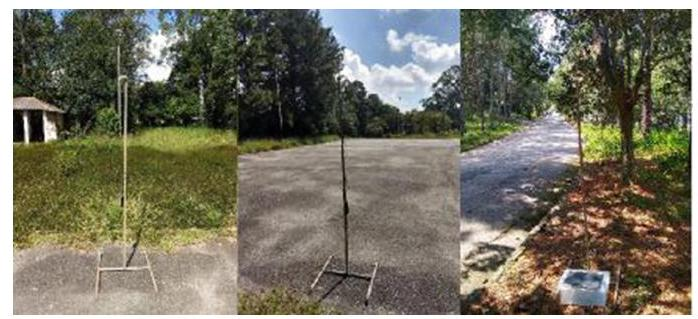
\includegraphics[max width=\textwidth]{2022_02_28_100dc43db44c8290ce2ag-05}
  \renewcommand{\figurename}{图}
  \caption{室外环境}
\end{figure}

\begin{figure}[H]
  \subfigure[距离]{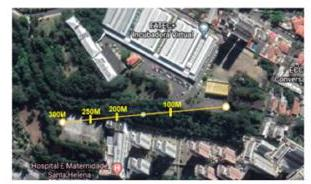
\includegraphics[width=0.5\columnwidth]{2022_02_28_100dc43db44c8290ce2ag-05(1)}}
  \subfigure[海拔]{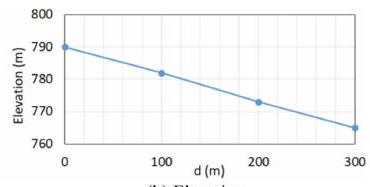
\includegraphics[width=0.5\columnwidth]{2022_02_28_100dc43db44c8290ce2ag-05(2)}}
  \renewcommand{\figurename}{图}
  \caption{室外环境的测量点位置和对应地形海拔}
\end{figure}

图6将RSSI作为$d$(距离)的函数,进行室外环境分析。对于LoRa,可以看出,当距离在$50$到$300\mathrm{m}$时:对于Config 1,RSSI从$-80$到$-110\mathrm{dBm}$,而对于Config 6,RSSI从$-85$到$-110\mathrm{dBm}$。由于LoRa设备的接收灵敏度为$-148\mathrm{dBm}$,因此系统在分析范围内正常运行(甚至可以覆盖更远的距离,如图所示)。对于Zigbee,距离在$50$到$250\mathrm{~m}$时,RSSI从$-57$到$-83\mathrm{dBm}$。然而,不可能在$300 \mathrm{~m}$测量RSSI,因为所有收到的数据包都出错了,表明接收信号的电平低于Zigbee设备$-102\mathrm{dBm}$的接收灵敏度。

\begin{figure}[H]
  \centering
  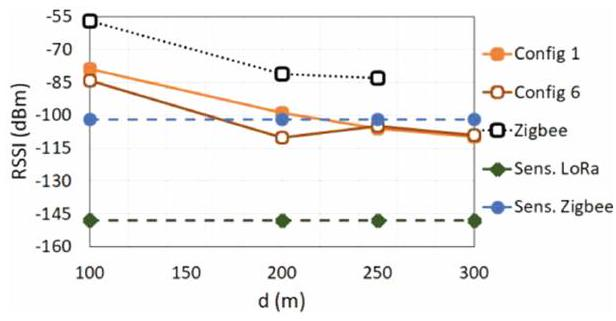
\includegraphics[max width=\textwidth]{2022_02_28_100dc43db44c8290ce2ag-06}
  \renewcommand{\figurename}{图}
  \caption{RSSI作为室外环境中$d$的函数}
\end{figure}

另一方面,图7显示了PER作为$d$(距离)的函数,对于Lora(Config 1 和Config 6)和 Zigbee在室外环境的分析结果。对于Lora,可以看出距离为$300\mathrm{~m}$时,Config 1达到最大PER值$3.0\%$,而Config 6达到最大PER值$2.5\%$。对于Zigbee,距离$200m$的PER为$34.71\%$,距离$250m$,PER低于$6.17\%$。这主要是环境的动态特性造成的,例如测试环境周围的人和车辆的流通。然而,距离$300\mathrm{~m}$时,Zigbee停止正常工作,所有收到的数据包都出错了(对应$100\%$的PER)。

\begin{figure}[H]
  \centering
  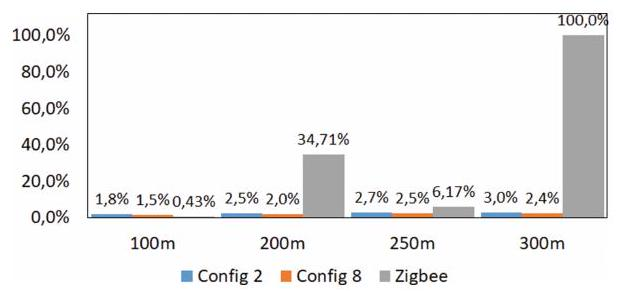
\includegraphics[max width=\textwidth]{2022_02_28_100dc43db44c8290ce2ag-06(1)}
  \renewcommand{\figurename}{图}
  \caption{PER作为室外环境中$d$的函数}
\end{figure}

\section{阴影传播模型}
为了将平均接收功率$\left(P_{RX}\right)$估计为$d$(距离)的函数,使用了具有灵活性、简单性和在实际测量时的可行性的影子传播模型($SPM$)。该模型基于修改后的自由空间模型,使用对数正态随机变量$X_{SH}$来表示在$\mathrm{dB}[6,10]$可以通过标准差$\sigma_{SH}$的值来量化的环境的阴影效应。$SPM$的$P_{RX}$可以表示为:
$$
P_{RX}(d)=P_{RX}\left(d_{0}\right)-10 \cdot \gamma \cdot \log _{10}\left(\frac{d}{d_{0}}\right)+X_{SH}
$$

其中:$d_{0}$是参考距离,$P_{RX}\left(d_{0}\right)$是在$d_{0}$处接收到的平均功率,$P_{RX}(d)$是在$d$中接收到的平均功率,$\gamma$是环境的传播系数。

表2显示了室内环境中LoRa(针对所有分析的配置)和Zigbee频带的$\gamma$和$\sigma_{SH}$的值,由对数回归方法[6]确定。表2得到室内环境的$\gamma$和$\sigma_{SH}$。

\begin{table}[H]
  \centering
  \renewcommand{\tablename}{表}
  \caption{获得室内环境中的$\gamma$和$\sigma_{SH}$值}
  \begin{tabular}{l|l|l}
  \hline
  Configurations & $\gamma$ & $\sigma_{SH}$ \\
  \hline
  Config 1 & $1.35$ & $3.86$ \\
  \hline
  Config 2 & $1.35$ & $4.38$ \\
  \hline
  Config 3 & $0.9$ & $5.10$ \\
  \hline
  Config 4 & $1.74$ & $4.07$ \\
  \hline
  Config 5 & $1.57$ & $4.54$ \\
  \hline
  Config 6 & $1.60$ & $4.60$ \\
  \hline
  Config 7 & $1.97$ & $4.86$ \\
  \hline
  Config 8 & $1.45$ & $3.13$ \\
  \hline
  Zigbee & $1.8$ & $3.9$ \\
  \hline
  \end{tabular}
\end{table}

图8显示了测量的$P_{RX}$和从SPM获得的分析室内环境的$P_{RX}$。为了使LoRa分析更清晰,不失一般性,图中只给出了Config 1曲线。分析结果,可以验证$P_{RX}$沿$d$发生了一些变化,主要是传输信号的半波长倍数多径分量的消除引起的。对于Zigbee,可以看出,测量的$P_{RX}$也由于多径分量的抵消而变化。需要注意的是,由于环境的物理限制(即$100\mathrm{~m}$ ),在距离大于临界距离$\left(D_{c}\right)$[6]时,无法获得$\gamma$和$\sigma_{SH}$的估计值。

\begin{figure}[H]
  \subfigure[LoRa(Config 1)]{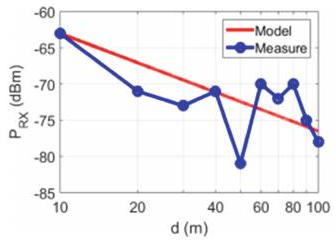
\includegraphics[width=0.5\columnwidth]{2022_02_28_100dc43db44c8290ce2ag-07}}
  \subfigure[Zigbee]{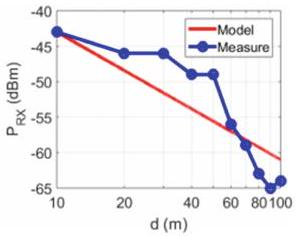
\includegraphics[width=0.5\columnwidth]{2022_02_28_100dc43db44c8290ce2ag-07(1)}}
  \renewcommand{\figurename}{图}
  \caption{$P_{R X}$作为室内环境中$d$的函数}
\end{figure}

反过来,图9显示了阴影分量对LoRa(Config 1)和Zigbee在室内环境中SPM获得的$P_{RX}$曲线的随机影响。测量的$P_{RX}$曲线也显示为参考。

\begin{figure}[H]
  \subfigure[LoRa(Config 1)]{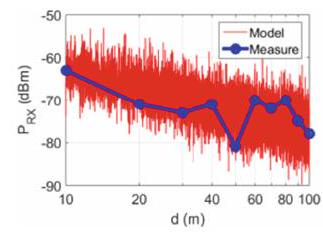
\includegraphics[width=0.5\columnwidth]{2022_02_28_100dc43db44c8290ce2ag-08}}
  \subfigure[Zigbee]{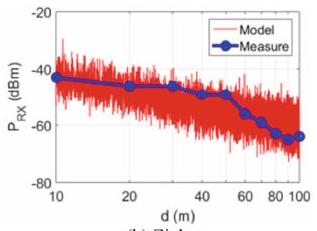
\includegraphics[width=0.5\columnwidth]{2022_02_28_100dc43db44c8290ce2ag-08(1)}}
  \renewcommand{\figurename}{图}
  \caption{在考虑阴影效应的情况下,$P_{R X}$作为室内环境中$d$的函数}
\end{figure}

表3显示了在分析的室外环境中Lora(Config 1和Config 6)和Zigbee获得的$\gamma$和$\sigma_{SH}$的值。可以看出,由于所分析环境的特征(例如,TX和RX之间的斜率,路径障碍物)以及测量使用距离大于$D_{c}$的一些点,获得了较高的$\gamma$。(例如,在$D_{c}$之外的点,$\gamma$由于地面反射而变为更高的值)[6]。

\begin{table}[H]
  \centering
  \renewcommand{\tablename}{表}
  \caption{获得室外环境中的$\gamma$和$\sigma_{SH}$值}
  \begin{tabular}{l|l|l}
  \hline
  Configurations & $\gamma$ & $\sigma_{S H}$ \\
  \hline
  Config 1 & $6.62$ & $0.44$ \\
  \hline
  Config 6 & $5.8$ & $4.73$ \\
  \hline
  Zigbee & $7.06$ & 2 \\
  \hline
  \end{tabular}
\end{table}

图10显示了在室外环境中从SPM测得的$P_{RX}$和$P_{RX}$的值。为简单起见,仅显示了Config 1的LoRa结果。可以看出,在所使用的模型和两个系统的测量值之间获得了良好的拟合。

\begin{figure}[H]
  \subfigure[LoRa(Config 1)]{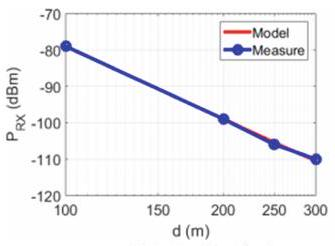
\includegraphics[width=0.5\columnwidth]{2022_02_28_100dc43db44c8290ce2ag-08(2)}}
  \subfigure[Zigbee]{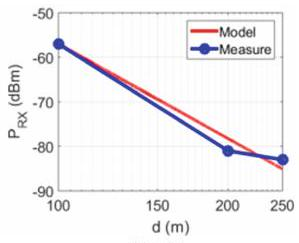
\includegraphics[width=0.5\columnwidth]{2022_02_28_100dc43db44c8290ce2ag-08(3)}}
  \renewcommand{\figurename}{图}
  \caption{$P_{R X}$作为室外环境中$d$的函数}
\end{figure}

另一方面,图11显示了阴影对室外环境中LoRa(Cinfig 1)和Zigbee从SPM获得的$P_{RX}$值曲线的影响。还显示了测量的$P_{R X}$值曲线。

\begin{figure}[H]
  \subfigure[LoRa(Config 1)]{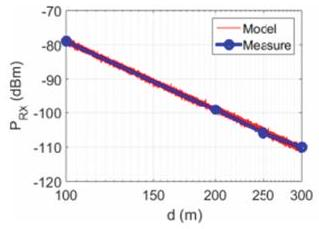
\includegraphics[width=0.5\columnwidth]{2022_02_28_100dc43db44c8290ce2ag-09}}
  \subfigure[Zigbee]{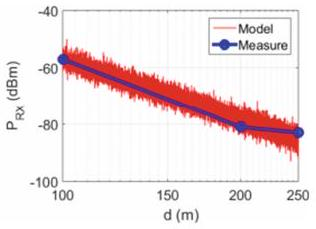
\includegraphics[width=0.5\columnwidth]{2022_02_28_100dc43db44c8290ce2ag-09(1)}}
  \renewcommand{\figurename}{图}
  \caption{考虑阴影效应的情况下,$P_{RX}$作为室外环境中$d$的函数}
\end{figure}

通过外推从SPM获得的$P_{R X}$曲线,根据接受灵敏度,可以获得所分析系统的最大范围的估计值。这样可以看出LoRa(Config 1)的最大范围是$1.1\mathrm{~km}$,而Zigbee的范围限制在$433.9\mathrm{~m}$。

\section{结论}
获得的结果表明:在室内和室外环境距离为$50\mathrm{~m}$的范围内,所评估的Zigbee系统具有比LoRa系统更好的性能。然而,在更深入的分析中,同样考虑到$50\mathrm{~m}$以上的覆盖范围,LoRa 被证明是低速率、低消耗和远程应用的最合适选择。工作在$915\mathrm{MHz}$频段的LoRa,比工作在$2.4\mathrm{GHz}$频段的Zigbee拥塞更少,并且具有更好的接收灵敏度,更广泛的覆盖范围和更好的信号质量,非常适合使用在工业4.0中。

\section{引用}
\begin{enumerate}
  \item Zhou Q, Zheng K, Hou L, Xing J, Xu R (2019) Design and implementation of open LoRa for IoT. IEEE Access 7:100,649-100,657

  \item Adame T, Bel A, Bellalta B (2019) Increasing LPWAN scalability by means of concurrent multiband IoT technologies: an industry $4.0$ use case. IEEE Access 7:46990-47010

  \item Aheleroff S, Xu X, Lu Y, Aristizabal M, Velásquez PJ, Joa B, Valencia Y (2020) IoT-enabled smart appliances under industry 4.0: a case study. Adv Eng Inform 43:101,043

  \item Sisinni E, Ferrari P, Fernandes Carvalho D, Rinaldi S, Marco P, Flammini A, Depari A (2020) LoRaWan range extender for industrial IoT. IEEE Trans Ind Inform 16(8):5607-5616

  \item El Chall R, Lahoud S, El Helou M (2019) LoRaWAN network: radio propagation models and performance evaluation in various environments in Lebanon. IEEE Internet Things J 6(2):2366-2378

  \item Casella IRS, Pereira AL (2016) A bioinspired propagation model for brazilian digital TV system based on MLP and RBF networks. IEEE Latin Am Trans 14:3941-3948

  \item Filsoof R, Bodine A, Gill B, Makonin S, Nicholson R (2014) Transmitting patient vitals over a reliable zigbee mesh network. In: 2014 IEEE Canada International Humanitarian Technology Conference, IHTC 2014, pp 1-5 8. Croce D, Gucciardo M, Mangione S, Santaromita G, Tinnirello I (2018) Impact of LoRa imperfect orthogonality: analysis of link-level performance. IEEE Commun Lett 22(4):796799

  \item Raposo D, Rodrigues A, Sinche S, Sá Silva J, Boavida F (2018) Industrial IoT monitoring: technologies and architecture proposal. Sensors 18(10):3568

  \item Cheung KW, Sau JHM, Murch RD (1998) A new empirical model for indoor propagation prediction. IEEE Trans Veh Technol 47(3):996-1001
\end{enumerate}

\end{document}